The method of manufactured solutions (MMS) was used to evaluate spatial
convergence rates of different schemes. A 1-D steady-state problem on
the domain $x\in(0,\frac{\pi}{4})$ was used with an MMS source of
\begin{equation}
  q(x) = v_x\cos(x) + \sigma(\sin(x) + u^{inc}) \eqc
\end{equation}
which leads to the following MMS solution:
\begin{equation}
  u(x) = \sin(x) + u^{inc} \eqp
\end{equation}

Figure \ref{fig:convergence} shows the convergence rates for each scheme
in the $L^1$ and $L^2$ norms. Both norms show the expected convergence
rates; the low-order scheme shows 1st-order convergence, and the high-order
schemes show 2nd-order convergence.

%-------------------------------------------------------------------------------
\begin{figure}[ht]
   \centering
   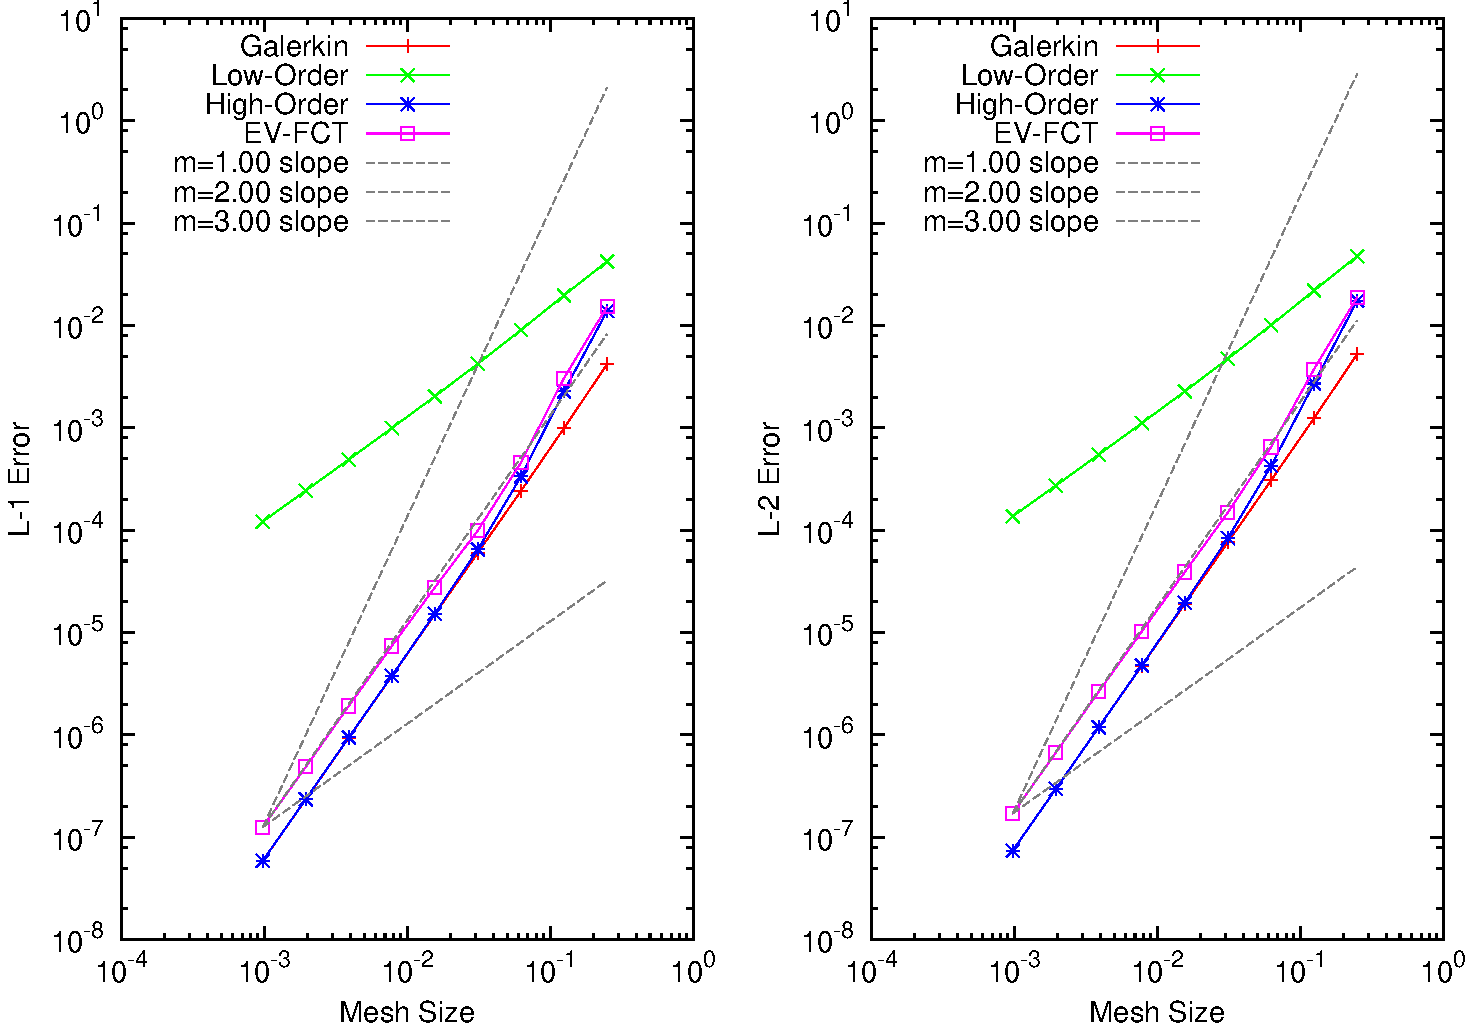
\includegraphics[width=0.9\textwidth]
     {\contentdir/results/transport/mms/convergence_smooth_FE.pdf}
   \caption{Comparison of Spatial Convergence Rates for a Smooth MMS Test Problem}
   \label{fig:convergence}
\end{figure}
%-------------------------------------------------------------------------------
